\documentclass[a4paper,11pt]{article}

\usepackage[utf8]{inputenc}
\usepackage[T1]{fontenc}
\usepackage[english,french]{babel}
	\frenchbsetup{SmallCapsFigTabCaptions=false}
\usepackage{indentfirst}
\usepackage[margin=2cm]{geometry}
\usepackage[table,kerneldraw,dvipsnames]{xcolor}
\usepackage{pdflscape}
\usepackage{rotating}

\usepackage{csquotes}
\usepackage[natbib=true,backend=biber,style=ieee,sort=none,sortcites=true,backref=true,backref=false,url=false,isbn=true,doi=true]{biblatex}
\DefineBibliographyExtras{french}{\restorecommand\mkbibnamefamily}
\addbibresource{references.bib}
\AtBeginBibliography{\small}

\usepackage{titlesec}
\titleformat{\section}[hang]{\Large\bfseries}{\thesection.~}{0pt}{}[]

\usepackage{fancyhdr}
\pagestyle{fancy}
\fancyhead{}
\fancyhead[C]{\footnotesize \itshape A. Huat / Projet de \DL (2018)}

\usepackage[nopostdot,nonumberlist,toc,acronyms]{glossaries}
\renewcommand{\glossarypreamble}{\small}

\usepackage{booktabs,array,longtable,tabularx}

\usepackage{menukeys}
\usepackage[shortcuts]{extdash}
\usepackage{enumitem}
%	\setlist{itemsep=0ex}
\usepackage{multicol}
\newenvironment{colfig}{\par\medskip\noindent\minipage{\linewidth}}{\endminipage\par\medskip}

\usepackage{float}
\usepackage{graphicx}
	% Centering figures by default
	\makeatletter
	\g@addto@macro\@floatboxreset{\centering}
	\makeatother
\usepackage{here}
\usepackage{placeins}
\usepackage[labelfont=bf,justification=justified,font=small,labelsep=period]{caption}
    \captionsetup[table]{singlelinecheck=false,name=Tableau}
% \usepackage{floatrow}
	\floatplacement{figure}{htbp}
	\floatplacement{table}{htbp}

\usepackage[colorlinks=true,plainpages=false,breaklinks=true,allcolors=NavyBlue]{hyperref}
\usepackage{fancyref}

\usepackage{listings,listingsutf8}
	\lstset{
		breaklines=true,
		deletekeywords={},
		frame=single,
		morekeywords={pour, chaque},
		tabsize=4,
		basicstyle=\scriptsize,
		escapeinside={lx*}{*lx}
}

% Maths

\usepackage{cool}
\usepackage{upgreek}
\usepackage{upref}
\usepackage{mathtools}
\usepackage{amsmath}
\usepackage{amsfonts}
\usepackage{amsthm}
\theoremstyle{definition}
\usepackage{amssymb}
\usepackage[scaled=1.]{rsfso}
\usepackage[scaled=1.,mathscr]{urwchancal}
\usepackage{stmaryrd}

% --------------------------------------
% Macros
% --------------------------------------

\newcommand{\fnhref}[2]{\href{#1}{#2}\footnote{\url{#1}}}

\newcommand{\TODO}[1]{\textsf{\color{orange}\bfseries TODO: #1}}

\newcommand{\cad}{c'est-à-dire}
\newcommand{\Cad}{C'est-à-dire}
\newcommand{\pex}{par exemple}
\newcommand{\Pex}{Par exemple}
\newcommand{\AH}{Alexandre Huat}
\newcommand{\eg}{\textit{e.g.}}
\newcommand{\ie}{\textit{i.e.}}
\newcommand{\etc}{\textit{etc.}}
\newcommand{\etal}{\textit{et al.}}
\newcommand{\vs}{\textit{vs.}}
\newcommand{\cf}{\textit{cf.}}
\newcommand{\Cf}{\textit{Cf.}}
\newcommand{\idem}{\textit{idem}}
\newcommand{\Idem}{\textit{Idem}}
\newcommand{\ibid}{\textit{ibid}}
\newcommand{\Ibid}{\textit{Ibid}}

\newcommand{\DL}{Deep Learning}

% Maths

% --------------------------------------
% Glossaire
% --------------------------------------

\makeglossaries

%%% Acronyms

\newacronym{eddp}{$(\epsilon, \delta)$-DP}{$(\epsilon, \delta)$--différentiellement confidentiel}

%%% Maths

% --------------------------------------
% Title
% --------------------------------------

\title{\textbf{Projet de \DL}\\« Differentially Private Releasing via Deep Generative Model »}
\author{\textbf{\AH}\\Master Science des Données\\INSA Rouen Normandie\\\texttt{alexandre.huat@insa-rouen.fr}}
\date{\today}

% ======================================

\begin{document}
\maketitle
\hrule

\begin{multicols}{2}
\section{Résumé}
Supposons un groupe de clients et un prestateur de services informatiques collectant et analysant leurs données (\eg\ classification d'images). Au cours des tâches d'analyses, le prestateur est amené à traiter des données sensibles. Afin de respecter la vie privée de ses clients, il doit trouver un moyen de traiter efficacement ces données tout en conservant leur confidentialité. C'est à cette problématique que répondent \citet{ref} par l'architecture dp-GAN de l'article résumé ici.

La \autoref{dp-gan_role} illustre le rôle de dp-GAN, qui est de générer des données synthétiques mais sémantiquement riches, \ie\ suffisamment représentatives des clients, sans violation de leur vie privée.
En introduction, les auteurs rappellent les défis à relever en apprentissage sous contrainte de confidentialité et présentent les apports de dp-GAN. En plus de sa capacité à générer une infinité de données, dp-GAN garantit l'anonymisation des données réelles par respect du principe de « confidentialité différentielle »\footnote{Synthétiqument, la confidentialité différentielle mesure la capacité d'un tiers à déduire des données privées des résultats d'un algorithme ; \cf\ exemple à \url{https://fr.wikipedia.org/wiki/Confidentialité_différentielle#Formalisation}.}.
Pour ce faire, dp-GAN applique au réseau adverse génératif de Wisserstein (WGAN) amélioré des mécanismes d'anonymisation à l'état de l'art, alors optimisés pour gagner en stabilité et en scalabilité.

En Section 2, Zhang \etal\ font un rappel théorique sur les GAN et justifient leur utilisation du WGAN amélioré par une plus grande stabilité et un plus court temps d'apprentissage que le GAN originel. Ils font également la définition formelle de la confidentialité différentielle et citent des propriétés associées dont bénéficient dp-GAN.

La Section 3 présente dp-GAN dans sa version basique et fournit son algorithme d'apprentissage (Algorithme 1). Pour assurer sa confidentialité, à chaque mise-à-jour, l'algorithme bruite le gradient du discriminateur (bruitage gaussien et seuillage), à partir duquel un pirate pourrait autrement reconstruire les données privées. Cette technique est communément utilisée dans la littérature. Une preuve théorique du niveau de confidentialité différentielle atteint par l'algorithme est également apportée.

Néanmoins, cette version de dp-GAN possède trois inconvénients : \begin{itemize}\item elle génère des données de faible qualité ; \item elle converge moins rapidement que le GAN non-confidentiel, voire diverge ; \item elle est rigide et n'exploite aucune ressource bonus, \eg\ des données publiques.\end{itemize} Pour palier ces défauts, la version avancée de dp-GAN implémente : \begin{itemize}\item un regroupement des paramètres du réseau pour un réglage fin et spécifique de leurs bruits respectifs ; \item un seuillage adaptatif du gradient, qui évolue au cours des itérations ; \item une initialisation des paramètres du réseau par pré-apprentissage sur les données publiques disponibles.\end{itemize} Ces améliorations boostent la vitesse de convergence et la confidentialité de dp-GAN. La Section 4 détaille l'algorithme de  cette version avancée (Algorithme 3).

S'en suit un rapport d'expériences sur trois bases célèbres et libres d'accès : \fnhref{http://yann.lecun.com/exdb/mnist/}{MNIST}, \fnhref{http://mmlab.ie.cuhk.edu.hk/projects/CelebA.html}{CelebA} et \fnhref{http://lsun.cs.princeton.edu/2015.html}{LSUN}. LSUN est ensuite divisée en deux bases, l'une labellisée (LSUN-L) et l'autre non-labellisée (LSUN-U). Les expériences sont réalisées avec TensorFlow mais le code n'est pas partagé par ses auteurs. Les paramètres testés sont cependant renseignés, entre autres, le ratio données publiques sur données privées est fixé à 2 contre 98 pour chaque base. Ainsi, la Section 5 propose une évaluation qualitative et quantitative des performances du système. De mon point de vue, les images générées par dp-GAN, quelle que soit la base, sont assez vraisemblables ; MNIST en particulier est très bien simulée.
Dans leur deux premières expériences, Zhang \etal\ comparent quantitativement la qualité des données générées par dp-GAN aux données réelles et à celles générées par le GAN non-confidentiel. dp-GAN performe légèrement moins bien pour les données labellisées (plus faible score d'Inception) comme pour les non-labellisées (plus grand score de Jensen-Schannon). Dans leur troisième expérience, les auteurs comparent les performances atteintes en classification sur LSUN-L après apprentissage sur : \begin{itemize}\item les données réelles seules ; \item les données réelles jointes aux données synthétisées par un GAN non-confidentiel ; \item les données réelles jointes aux données synthétisées par dp-GAN.\end{itemize} Il en ressort que l'apprentissage avec les données synthétiques permet systématiquement une diminution des taux d'erreurs (jusqu'à $-3.3 \%$ pour dp-GAN, contre $-7.7 \%$ pour le GAN non-confidentiel). Quatrièmement, en terme de score d'Inception et de Jensen-Schannon, une ultime expérimentation valide l'efficacité des stratégies d'optimisations dont bénéficie dp-GAN avancé.

Dernièrement, les auteurs consacrent une section aux travaux similaires de la littérature. Puis, ils concluent en rappelant l'intérêt et les améliorations apportées par dp-GAN et, enfin, ouvrent la discussion sur la limite que l'architecture n'a été testée que sur des images – une évaluation sur d'autres types de données (\eg\ texte) étant bienvenue.
\end{multicols}

\begin{figure}
    \centering
    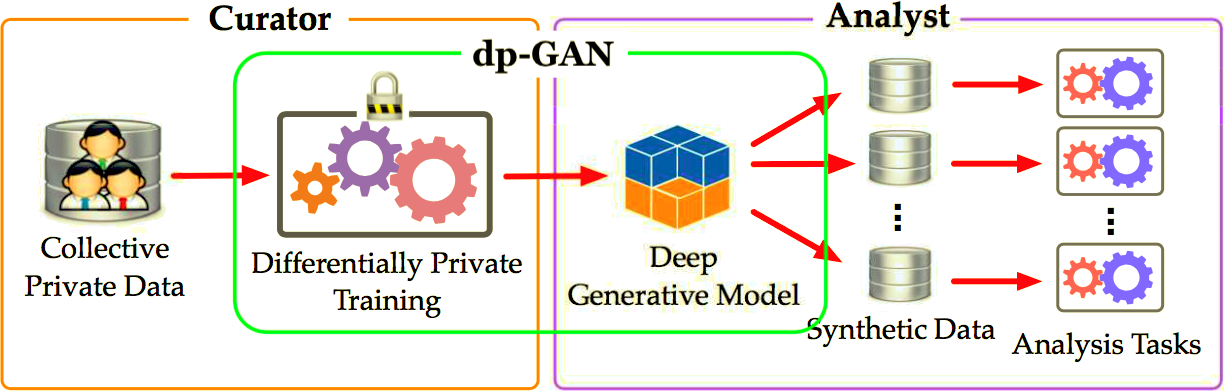
\includegraphics[width=0.7\textwidth]{dp-gan_role.png}
    \captionof{figure}{La place de dp-GAN dans la chaîne de traitement des données confidentielles. Le « \textit{curator} » est l'entité qui anonymise les données pour l'\textit{analyst}.}
    \label{dp-gan_role}
\end{figure}

\section{Implémentation}
Le véritable défi de ce projet est l'implémentation de dp-GAN basique. En effet, son implémentation m'apprendra les fonctionnements détaillés de WGAN et d'un « agent comptable de la confidentialité » \citep{pinq}. En revanche, dp-GAN avancé ne consiste qu'en l'enrichissement de dp-GAN basique d'un apprentissage sur des données publiques et d'un clustering hiérarchique des paramètres du réseau. Or, comptant de plus ma formation en apprentissage statistique et profond, ces opérations ne présentent pas de plus-value pédagogique. Sachant le temps allouable au projet, il m'apparaît raisonnable de me concentrer sur l'implémentation de dp-GAN basique, testée sur MNIST, CelebA et/ou LSUN.

GitHub : \url{https://github.com/alexandrehuat/dp-gan}.

\printbibliography[title=Références,heading=bibintoc]

\end{document}
